 %***************************************************************************%
 % Thesis presentation                                                       %
 %                                                                           %
 %                                                                           %
 %                        B A C H E L O R   T H E S I S                      %
 %                                                                           %
 %                                                                           %
 %  Title:           Template for Making Presentation with LaTeX             %
 %                                                                           %
 %  Author:                         Andrey Popov                             %
 %                                                                           %
 %  Supervisor:                     MSc. A. Popov                            %
 %                                                                           %
 %  Date:                            29.08.2007                              %
 %                                                                           %
 %***************************************************************************%

 %   Template - Institute of Control Systems, Hamburg University of Technology
 %
 %   A. Popov
 %
 %   Updates:  AP: 29.08.2007;  AP: 17.09.2007; AP: 16.06.2009
 %
 %   Version 0.3


 %##########################################
 %     R E A D      M E     F I R S T  !
 %##########################################
 % beamer package and manual can be downloaded from  %
 % http://tug.ctan.org/cgi-bin/ctanPackageInformation.py?id=powerdot
 %
 % Possible compilation processes:
 % LaTeX -> DVI -> PS -> PDF   [recomended]
 % LaTeX -> pdfTeX -> PDF
 %##########################################


 %------------------------------------------
 % INFO:   Presentation Time
 %------------------------------------------
 % Studienarbeit:                     20 min
 % Bachelor thesis, Master thesis,
 % Diplomarbeit:                      30 min 
 %------------------------------------------


 %%################ Document  settings ###################
\documentclass{beamer}

\mode<presentation>
{
  \usetheme{RT}
  \setbeamercovered{transparent}
  \usecolortheme{RT}
}
\usefonttheme{professionalfonts} 	% optional

\setbeamertemplate{footline}[frame number]{}


 %%######## Choose LANGUAGE

 %%% English
    \usepackage[english]{babel}		% comment if cause of errors
    \selectlanguage{english}		% (due to MikTex - babel versions)

 %%% German
%    \usepackage[english,ngerman]{babel}
%    \selectlanguage{ngerman}
   % %% In some cases you might need that
   % \usepackage{german}
    \usepackage[latin1]{inputenc}
    
% math environments and more by the AMS 
\PassOptionsToPackage{fleqn}{amsmath}		
 \usepackage{amsmath}

%When using tikZ one must also use the color package.
\PassOptionsToPackage{usenames,dvipsnames}{color}
 \usepackage{color}
%This package lets you compile tikz graphics.
 \usepackage{tikz}
 \usepackage{pgfplots}
 \usetikzlibrary{decorations.markings}
 \usepackage{standalone}

%Code Listings
\usepackage{listings} 
\lstset{language=Matlab,
    keywordstyle=\color{blue},%\bfseries,
    basicstyle=\small\ttfamily,
    identifierstyle=\color{blue},
    %commentstyle=\color{green}\ttfamily,
    stringstyle=\rmfamily,
    numbers=none,%left,%
    numberstyle=\scriptsize,%\tiny
    stepnumber=5,
    numbersep=8pt,
    showstringspaces=false,
    breaklines=true,
    frameround=ftff,
    frame=single,
    belowcaptionskip=.75\baselineskip
    %frame=L
} 


 %%######## Chose FONT
\usepackage[T1]{fontenc}
% Note that the encoding and the font should match. If T1
% does not look nice, try deleting the line with the fontenc.

%\usepackage[utf8]{inputenc}
\usepackage{times}



 %%######## GRAPHICS Options
\graphicspath{{figures/}}				% Define the path to the figures

\usepackage{ifpdf}

\ifpdf % pdfTeX
	\DeclareGraphicsExtensions{.pdf,.png,.jpg,.gif,.pdftex}
	\DeclareGraphicsRule{.pdftex}{pdf}{*}{}	% for xfig exported files
	\newcommand{\xfig}[2]{\scalebox{#1}{\input{"../figures/#2.pdftex_t"}}} % XFIG
\else % DVI
	\DeclareGraphicsExtensions{.eps,.pstex}
	\DeclareGraphicsRule{.pstex}{eps}{*}{}		% for xfig exported files
	\newcommand{\xfig}[2]{\scalebox{#1}{\input{"../figures/#2.pstex_t"}}} % XFIG
	%\usepackage{psfrag}		% might be useful
\fi

 % Other figures (e.g., MATLAB  EPS or PDF figures)
\newcommand{\afig}[2]{\includegraphics[scale=#1]{#2}}

 % figures defined in TeX files
\newcommand{\tfig}[2]{\scalebox{#1}{\input{"#2.tex"}}}



 %%######## Logos only on Title page
\titlegraphic{\vspace{0.1cm}\includegraphics[height=0.8cm]{../figures/kuLeuven.png} \hfill \includegraphics[height=1.9cm]{../figures/numLinLogo.png}}




 %%######## Other FUNCTIONS

\newcommand{\vs}[1]{\vspace{#1mm}}

\newcommand{\bbma} {\begin{bmatrix} }
\newcommand{\ebma} {\end{bmatrix}}

 % Some color definitions
\setbeamercolor{greenhead}{fg=white,bg=green!80!black}%
\setbeamercolor{greenbody}{fg=black,bg=green!50!white}%

\setbeamercolor{redhead}{fg=white,bg=red!80!black}%
\setbeamercolor{redbody}{fg=black,bg=red!50!white}%
    % make all adjustments to language and packages here


\title{The Tortoise and the Hare, Restart GMRES}

\author[Moritz Wolter]{Moritz Wolter \texorpdfstring{\\}{} {\small\texttt{moritzalexander.wolter @ student.kuleuven.de}}}


%\institute{
%	Ku Leuven\\ Numerical Linear Algebra 
%}

%\date[\today]{Template presentation \\ 19.08.2007}
 % (optional, should be abbreviation of conference name)

\subject{Pseudospektren}

% This makes a table of contents at the begining of each section. This is used to show where you are in the presentation and for navigation.
\AtBeginSection[]
{
  \begin{frame}<beamer>{Contents}
    \tableofcontents[currentsection,hideallsubsections]
  \end{frame}
}


%#######################BEGIN THE PRESENTATION #######################
\begin{document}

 % Title page
\begin{frame}\titlepage
\end{frame}

 % Table of contents (used also for navigation)
\begin{frame}{Contents}
  \tableofcontents[hideallsubsections]
\end{frame}

% Delete this, if you do not want the table of contents to pop up at
% the beginning of each subsection:
\AtBeginSection[]
{
  \begin{frame}<beamer>{Contents}
    \tableofcontents[currentsection,hideallsubsections]
  \end{frame}
}
\section{Recap GMRES}
\begin{frame}
\frametitle{Recap \texttt{GMRES(m)}}
  \begin{enumerate}
  \item Start: Choose $x_0$ and compute $r_0 = f - Ax_0$ and $v_1 = r_0/\|r_0\|$ 
  \item Iterate: For j = 1,2,\dots,m do \\
        $h_{i,j} = (Av_j,v_i), i = 1,\dots,j $\\
        $\hat{v}_{j+1} = Av_j  - \sum_{i=1}^{j} h_{i,j}v_{i}$ \\
        $h_{j+1,j} = \| \hat{v}_{j+1} \| $, and \\
        $v_{j+1} =  \hat{v}_{j+1} / {h}_{j+1,j} $ \\
  \item Form the approximate solution:
        $x_m = x_0 + V_m y_m$ where $y_m$ minimizes $\| \beta e_1 - H_m y \|, y\in \mathbb{R}^m$
  \item Restart:
        Compute $r_m = f - Ax_m$; if satisfied stop, else
        $x_0 = x_m, v_1 = r_m/\|r_m\|$
  
  \end{enumerate}
  
  
\end{frame}

\section{The Problem}
\begin{frame}
  \frametitle{GMRES(\texttt{m}) convergence}
	\begin{figure}
		\input{../images/randGMRESTwoInOne.tex}
		\caption{GMRES(\texttt{m}) convergence on large random matrix $\mathbf{A}$ of dimension 60 with $\mathbf{b} = [0 \dots 1 \dots 0]^T$ in blocks of 20 each.}
    \end{figure}
  
\end{frame}



\begin{frame}
\begin{eqnarray}
\mathbf{A}_1 =
\begin{pmatrix}
1 & 1 & 1 \\
0 & 1 & 3 \\
0 & 0 & 1 \\
\end{pmatrix}
\mathbf{b}_1 =
\begin{pmatrix}
2 \\ -4 \\ 1 \\
\end{pmatrix} \\
\mathbf{A}_2 =
\begin{pmatrix}
1 & 2 & -2 \\
0 & 2 & 4 \\
0 & 0 & 3 \\
\end{pmatrix}
\mathbf{b}_2 =
\begin{pmatrix}
3 \\ 1 \\ 1 \\
\end{pmatrix}
\end{eqnarray}
\end{frame}


\begin{frame}
	\frametitle{Gmres convergence}	
	\begin{figure}
		% This file was created by matlab2tikz.
% Minimal pgfplots version: 1.3
%
%The latest updates can be retrieved from
%  http://www.mathworks.com/matlabcentral/fileexchange/22022-matlab2tikz
%where you can also make suggestions and rate matlab2tikz.
%
\documentclass[tikz]{standalone}
\usepackage{pgfplots}
\usepackage{grffile}
\pgfplotsset{compat=newest}
\usetikzlibrary{plotmarks}
\usepackage{amsmath}

\begin{document}
\definecolor{mycolor1}{rgb}{0.00000,0.44700,0.74100}%
\definecolor{mycolor2}{rgb}{0.85000,0.32500,0.09800}%
%
\begin{tikzpicture}

\begin{axis}[%
width=2.25in,
height=2.25in,
at={(0.744792in,0.446875in)},
scale only axis,
xmin=0,
xmax=35,
ymode=log,
ymin=1e-20,
ymax=1,
yminorticks=true,
legend style={legend cell align=left,align=left,draw=white!15!black}
]
\addplot [color=mycolor1,solid,line width=2.0pt]
  table[row sep=crcr]{%
1	1\\
2	0.925820099772552\\
3	0.654653670707977\\
4	2.22044604925031e-16\\
5	2.22044604925031e-16\\
6	2.22044604925031e-16\\
7	2.22044604925031e-16\\
8	2.22044604925031e-16\\
9	2.22044604925031e-16\\
10	2.22044604925031e-16\\
11	2.22044604925031e-16\\
12	2.22044604925031e-16\\
13	2.22044604925031e-16\\
14	2.22044604925031e-16\\
15	2.22044604925031e-16\\
16	2.22044604925031e-16\\
17	2.22044604925031e-16\\
18	2.22044604925031e-16\\
19	2.22044604925031e-16\\
20	2.22044604925031e-16\\
21	2.22044604925031e-16\\
22	2.22044604925031e-16\\
23	2.22044604925031e-16\\
24	2.22044604925031e-16\\
25	2.22044604925031e-16\\
26	2.22044604925031e-16\\
27	2.22044604925031e-16\\
28	2.22044604925031e-16\\
29	2.22044604925031e-16\\
30	2.22044604925031e-16\\
31	2.22044604925031e-16\\
};
\addlegendentry{GMRES(1)};

\addplot [color=mycolor2,solid,line width=2.0pt]
  table[row sep=crcr]{%
1	1\\
2	0.462910049886276\\
3	0.377189160453301\\
4	0.376548629114522\\
5	0.376512989917567\\
6	0.37650248885891\\
7	0.376498558527189\\
8	0.376497022258869\\
9	0.376496407650134\\
10	0.376496158161928\\
11	0.376496055944867\\
12	0.376496013816942\\
13	0.376495996388108\\
14	0.376495989159931\\
15	0.3764959861575\\
16	0.376495984909088\\
17	0.376495984389657\\
18	0.376495984173445\\
19	0.376495984083423\\
20	0.376495984045934\\
21	0.376495984030321\\
22	0.376495984023818\\
23	0.376495984021109\\
24	0.376495984019981\\
25	0.376495984019511\\
26	0.376495984019315\\
27	0.376495984019233\\
28	0.376495984019199\\
29	0.376495984019185\\
30	0.376495984019179\\
31	0.376495984019177\\
};
\addlegendentry{GMRES(2)};

\end{axis}
\end{tikzpicture}%
\end{document}
		\caption{\texttt{GMRES} convergence on matrix $\mathbf{A}_1. $}
    \end{figure}
\end{frame}

\begin{frame}
	\begin{figure}
			% This file was created by matlab2tikz.
% Minimal pgfplots version: 1.3
%
%The latest updates can be retrieved from
%  http://www.mathworks.com/matlabcentral/fileexchange/22022-matlab2tikz
%where you can also make suggestions and rate matlab2tikz.
%
\documentclass[tikz]{standalone}
\usepackage{pgfplots}
\usepackage{grffile}
\pgfplotsset{compat=newest}
\usetikzlibrary{plotmarks}
\usepackage{amsmath}

\begin{document}
\definecolor{mycolor1}{rgb}{0.00000,0.44700,0.74100}%
\definecolor{mycolor2}{rgb}{0.85000,0.32500,0.09800}%
%
\begin{tikzpicture}

\begin{axis}[%
width=2.25in,
height=2.25in,
at={(0.744792in,0.446875in)},
scale only axis,
xmin=0,
xmax=35,
ymode=log,
ymin=1e-20,
ymax=1,
yminorticks=true,
legend style={legend cell align=left,align=left,draw=white!15!black}
]
\addplot [color=mycolor1,solid,line width=2.0pt]
  table[row sep=crcr]{%
1	1\\
2	0.925820099772552\\
3	0.654653670707977\\
4	2.22044604925031e-16\\
5	2.22044604925031e-16\\
6	2.22044604925031e-16\\
7	2.22044604925031e-16\\
8	2.22044604925031e-16\\
9	2.22044604925031e-16\\
10	2.22044604925031e-16\\
11	2.22044604925031e-16\\
12	2.22044604925031e-16\\
13	2.22044604925031e-16\\
14	2.22044604925031e-16\\
15	2.22044604925031e-16\\
16	2.22044604925031e-16\\
17	2.22044604925031e-16\\
18	2.22044604925031e-16\\
19	2.22044604925031e-16\\
20	2.22044604925031e-16\\
21	2.22044604925031e-16\\
22	2.22044604925031e-16\\
23	2.22044604925031e-16\\
24	2.22044604925031e-16\\
25	2.22044604925031e-16\\
26	2.22044604925031e-16\\
27	2.22044604925031e-16\\
28	2.22044604925031e-16\\
29	2.22044604925031e-16\\
30	2.22044604925031e-16\\
31	2.22044604925031e-16\\
};
\addlegendentry{GMRES(1)};

\addplot [color=mycolor2,solid,line width=2.0pt]
  table[row sep=crcr]{%
1	1\\
2	0.462910049886276\\
3	0.377189160453301\\
4	0.376548629114522\\
5	0.376512989917567\\
6	0.37650248885891\\
7	0.376498558527189\\
8	0.376497022258869\\
9	0.376496407650134\\
10	0.376496158161928\\
11	0.376496055944867\\
12	0.376496013816942\\
13	0.376495996388108\\
14	0.376495989159931\\
15	0.3764959861575\\
16	0.376495984909088\\
17	0.376495984389657\\
18	0.376495984173445\\
19	0.376495984083423\\
20	0.376495984045934\\
21	0.376495984030321\\
22	0.376495984023818\\
23	0.376495984021109\\
24	0.376495984019981\\
25	0.376495984019511\\
26	0.376495984019315\\
27	0.376495984019233\\
28	0.376495984019199\\
29	0.376495984019185\\
30	0.376495984019179\\
31	0.376495984019177\\
};
\addlegendentry{GMRES(2)};

\end{axis}
\end{tikzpicture}%
\end{document}
			\caption{\texttt{GMRES} convergence on matrix $\mathbf{A}_2$.}
	\end{figure}
\end{frame}



\section{The problem in 2d}
\begin{frame}
	\frametitle{Convergence in a two dimesional plane}
	\begin{figure}
	\centering
	\includegraphics[width=0.45\linewidth]{../images/fig4Matp2}
	\includegraphics[width=0.45\linewidth]{../images/fig4Matp1}
	\caption{Residual magnitude Plot for matrix $\mathbf{A}_2, \mathbf{b}_2$, as seen in the Embree paper for GMRES(1)(left) and GMRES(2)(right) in figure 4.}
	\label{fig:fig4}
	\end{figure}
\end{frame}

\begin{frame}
\frametitle{Convergence in a two dimesional plane}
\begin{figure}
\centering
\includegraphics[width=0.45\linewidth]{../images/fig2Matp1}
\includegraphics[width=0.45\linewidth]{../images/fig2Matp2}
\caption{Residual magnitude Plot for the $\mathbf{A}_1,\mathbf{b}_1 $ pair, as seen in the Embree paper GMRES(1)(left) and GMRES(2)(right) in figure two.}
\label{fig:fig2}
\end{figure}
\end{frame}


\begin{frame}
\frametitle{Conditioning makes a difference.}
	\begin{figure}
	\centering
	\includegraphics[width=0.45\linewidth]{../images/Am0p35eyeGMRES1}
	\includegraphics[width=0.45\linewidth]{../images/Am0p35eyeGMRES2}
	\caption{\texttt{GMRES(1)} and \texttt{GMRES(2)} convergence on $\mathbf{A} - 0.35 \cdot \mathbf{I}$. $\kappa(\mathbf{A}) = 14.2950$ changes to $\kappa(\mathbf{A} - 0.35 \cdot \mathbf{I}) = 39.1873$.} 
	\label{fig:modA}
	\end{figure}
\end{frame}

\begin{frame}
\frametitle{A random matrix.}
\begin{equation}
\mathbf{R} = \begin{pmatrix}
-0.3034 &   0.8884 &  -0.8095 \\
 0.2939 &  -1.1471 &  -2.9443 \\
-0.7873 &  -1.0689 &   1.4384 \\
\end{pmatrix} 
\end{equation}
\end{frame}
%b comes from the complex plane!

\begin{frame}
\begin{figure}
\centering
\includegraphics[width=0.45\linewidth]{../images/randAGMRES1}
\includegraphics[width=0.45\linewidth]{../images/randAGMRES2}
\caption{Convergence of \texttt{GMRES(1)}(left) and \texttt{GMRES(2)}(right) for the random matrix $\mathbf{R}$. $\kappa(\mathbf{R}) = 5.1025$ }
\label{fig:randAGMRES2}
\end{figure}
\end{frame}

\begin{frame}
\begin{figure}
\centering
\includegraphics[width=0.45\linewidth]{../images/randAp2eyeGMRES1}
\includegraphics[width=0.45\linewidth]{../images/randAp2eyeGMRES2}
\caption{Convergence results for $\mathbf{R} + 2\mathbf{I}$. $\kappa(\mathbf{R} + 2\mathbf{I}) = 77.5446$. }
\label{fig:randAp2eyeGMRES2}
\end{figure}
\end{frame}
\begin{frame}
\begin{figure}
\centering
\includegraphics[width=0.45\linewidth]{../images/randAp3eyeGMRES2}
\includegraphics[width=0.45\linewidth]{../images/randAp3eyeGMRES2}
\caption{Convergence results for $\mathbf{R} + 3\mathbf{I}$. $\mathbf{R} + 3\mathbf{I} = 6.4262$.}
\label{fig:randAp3eyeGMRES2}
\end{figure}
\end{frame}


\begin{frame}
 \begin{equation}
 \mathbf{C} = \begin{pmatrix}
 1 & -2 \\
 0 & 1 \\
 \end{pmatrix}
 \;\;\;
 \mathbf{r_0} = \begin{pmatrix} \xi \\ \eta \end{pmatrix}
 \end{equation}
\end{frame}

\begin{frame}
\begin{figure}
\centering
\includegraphics[width=0.45\linewidth]{../images/twoDPaper}
\includegraphics[width=0.45\linewidth]{../images/twoDZoom}
\caption{A plot of the convergence plain for the matrix $\mathbf{C}$ proposed at the end of Embree's paper. With zoom on an interesting region.}
\label{fig:twoDZoom}
\end{figure}
\end{frame}

\section{More on the noise}
\begin{frame}
\begin{figure}
\centering
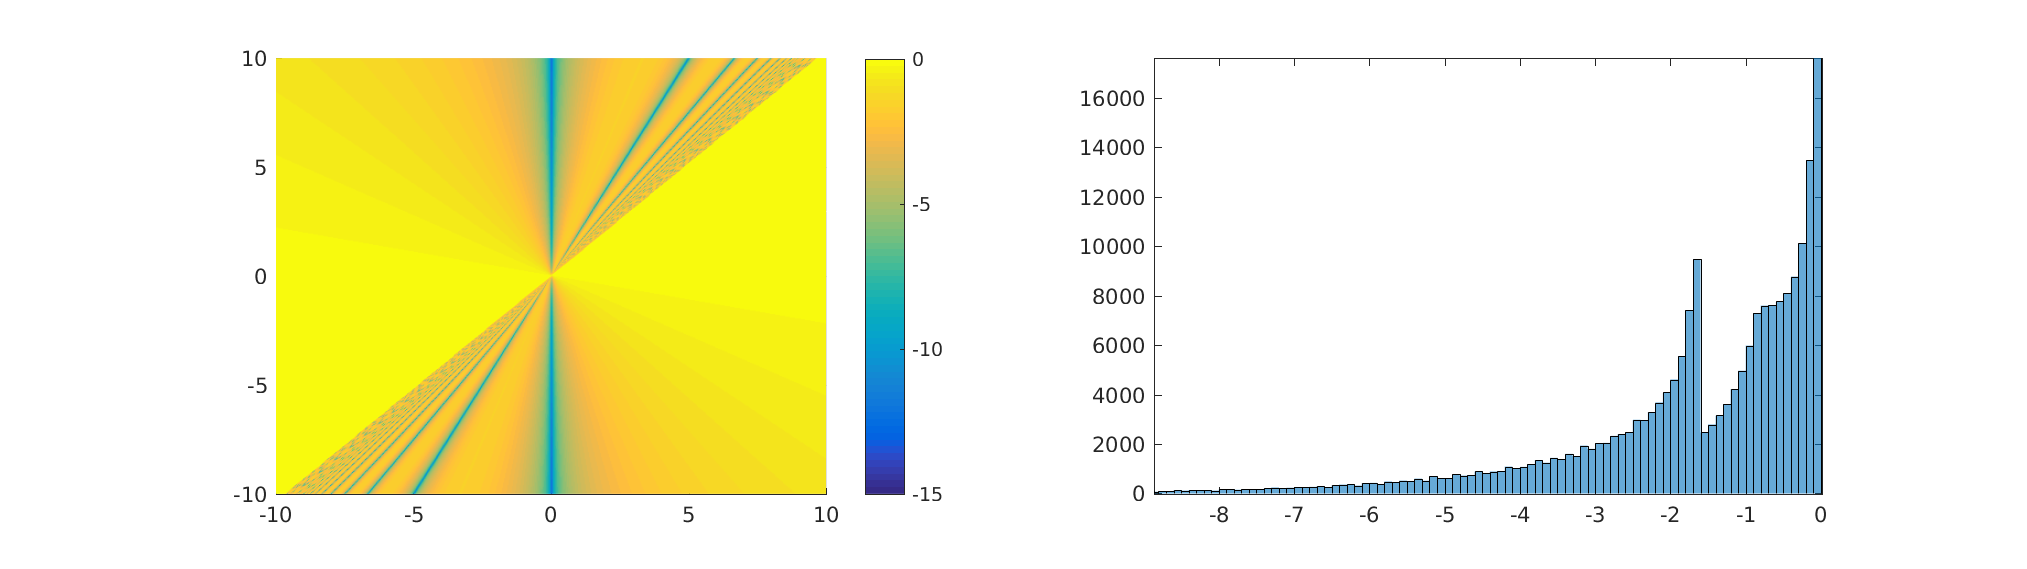
\includegraphics[width=1\linewidth]{../images/gmresCHist}
\caption{Convergence Plain and error histogram for matrix $\mathbf{C}$.}
\end{figure}
\end{frame}


\begin{frame}
\begin{itemize}
\item  $\mathcal{D}_1 = 10^{-1} + \| \mathcal{N}(0,2.5 \cdot 10^{-3}) \| $ \\
\item  $\mathcal{D}_2 = 10^{-5} + \| \mathcal{N}(0,2.5 \cdot 10^{-3}) \| $ \\
\end{itemize}

\begin{figure}
\centering
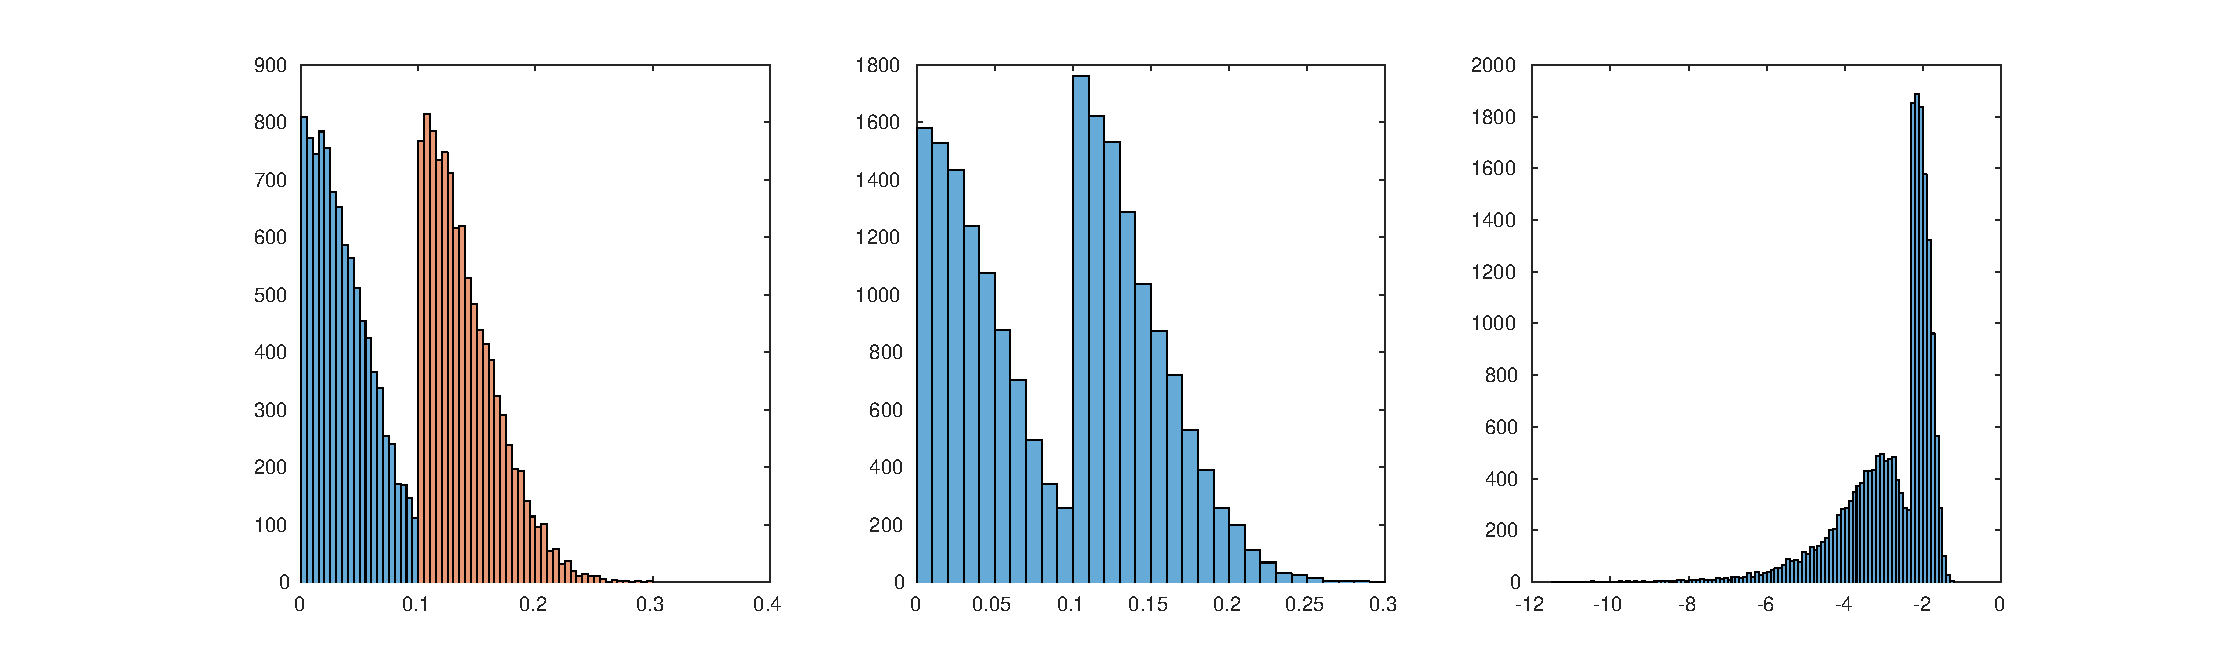
\includegraphics[width=1\linewidth]{../images/randnHist}
\caption{Plots of the distributions generated by
\texttt{d1 = 0.00001 + 0.05*abs(randn(10000,1));
d2 = 0.1 + 0.05*abs(randn(10000,1));} . The last plot is on a semilogarithmic scale. }
\end{figure}
\end{frame}

\begin{frame}
\begin{figure}
\centering
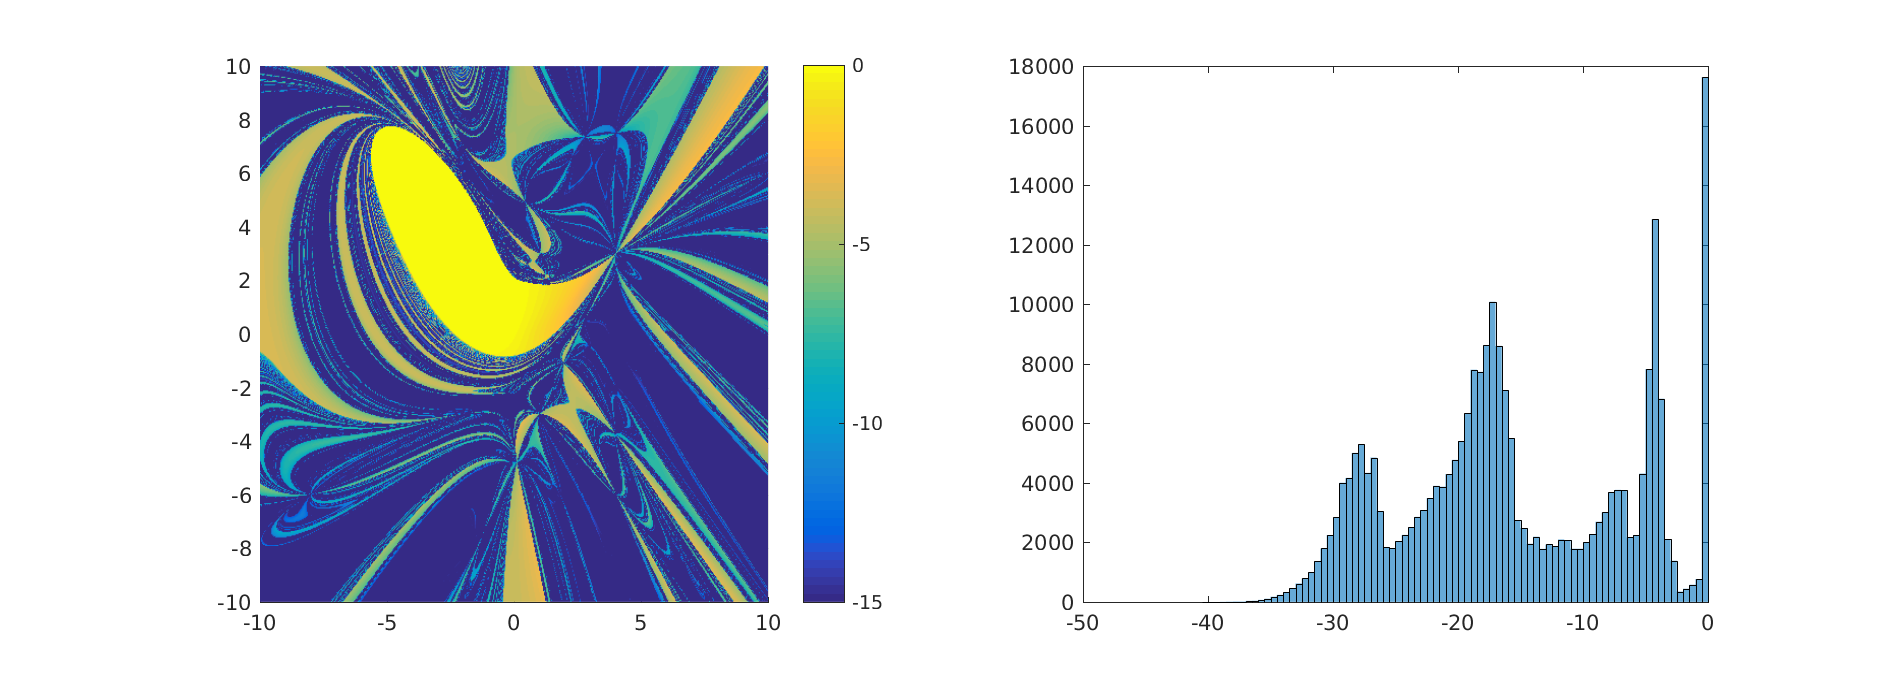
\includegraphics[width=1\linewidth]{../images/gmresBHist}
\caption{Convergence Plain and error histogram for matrix $\mathbf{B}$.}
\end{figure}
\end{frame}

\section{Stagnation condition}
\begin{frame}
\centering
\frametitle{Recurrence for \texttt{gmres(1)}.}
\begin{equation}
\mathbf{r}_{k + 1}^{(1)} = \mathbf{r}_k^{(1)} - \frac{\mathbf{r}_k^{(1)T} \mathbf{A} \mathbf{r}_k^{(1)}}{\mathbf{r}_k^{(1)T} \mathbf{A}^T \mathbf{A} \mathbf{r}_k^{(1)}} \mathbf{A} \mathbf{r}_k^{(1)}
\end{equation}
$\Rightarrow$ \texttt{gmres(1)} must stagnate if $\mathbf{r}_k^{(1)T} \mathbf{A} \mathbf{r}_k^{(1)} = 0$.
\end{frame}

\begin{frame}
\begin{figure}
\frametitle{Matrix $\mathbf{A}$}
\centering
\includegraphics[width=0.7\linewidth]{../images/gmresOneConvA}
\caption{Region of guaranteed convergence with \texttt{gmres(1)} on matrix $\mathbf{A}$.}
\label{fig:gmresOneConvA}
\end{figure}
\end{frame}

\begin{frame}
\begin{figure}
\frametitle{Matrix $\mathbf{B}$}
\centering
\includegraphics[width=0.7\linewidth]{../images/gmresOneConvB}
\caption{Region of guaranteed convergence with \texttt{gmres(1)} on matrix $\mathbf{B}$.}
\label{fig:gmresOneConvB}
\end{figure}
\end{frame}

\end{document}
